\chapter{FEA data management}
\label{chapter:data-management}

Together with growing complexity of finite element calculations, the importance of management of data produced by the calculations is increasingly emphasized in both industrial and research communities. As information is shared between multiple users, moved from one computer to another, and further transformed to enable different views over the data to enable inpterpretation of the information. Definition of persistent and standard representation of the data is therefore required as well as the corresponding data access system architecture that allows to query the data.

\section{System architecture}
\label{sec:system-architecture}

The prototype implementation of the FEA data management system is designed as a collaborative framework that can be accessed by users from different client devices. Figure \ref{fig:FEA-architecture} depicts the schema of the system architecture. System consists of several independent modules. The FEM calculation itself runs on a remote server as one of micro-services\footnote{TODO: micro-services} along with mesh generation service, results processing service, etc. These services are controlled by the application service that provides interface to the client applications in form of REST-ful web API\footnote{TODO: REST; REST-ful service; REST web API.}.

\begin{figure}[H]
    \centering
    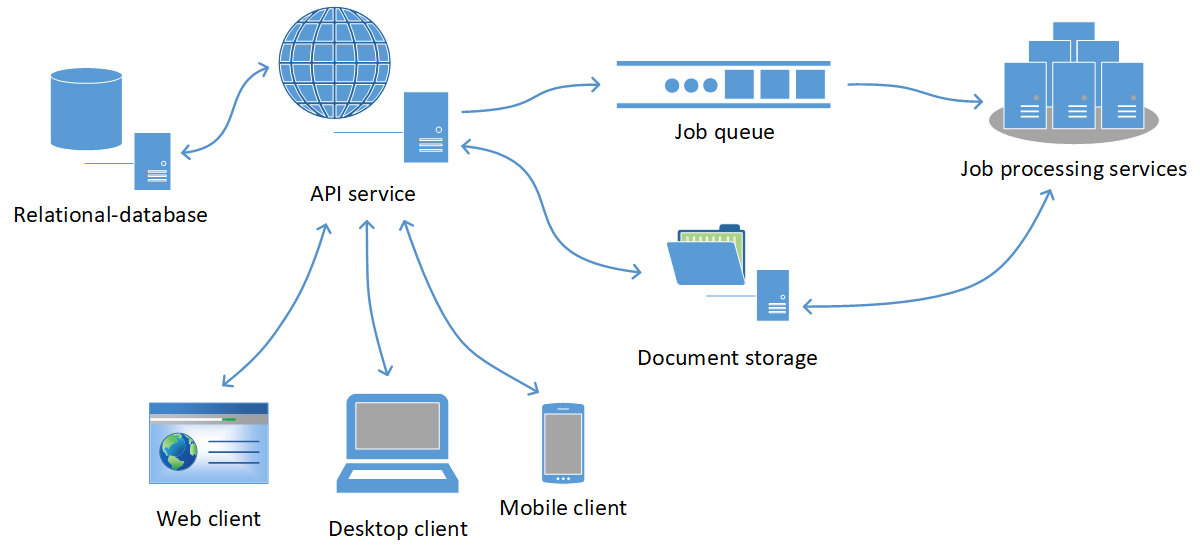
\includegraphics[width=\textwidth]{figures/chapter-data-management/FEA-architecture}
    \decoRule
    \caption{FEA system architecture.}
    \label{fig:FEA-architecture}
\end{figure}

The architecture relies on an abstraction provided by Platform-as-a-Service\footnote{PaaS. TODO: These services can be carried in a public cloud or on-premises. ...} computing model. No service component is tied directly to a specific machine. Hardware resources are allocated when they are needed by a service infrastructure controller. This makes the scaling and deployment of components easier and allows to focus on the problem domain instead of solving server configuration and networking issues.

The system contains two types of data storage. The relational-database type of storage is intended to store basic project-related data such as description of simulations, links to the simulation resources, information about the owner and other colaborating users, etc. The input to the FEA -- geometrical model, attribute assignments, and analysis parameters -- can also be stored in a relational database, eventhough, storing this complex type of information in the SQL database is questionable and has its drawbacks\footnote{TODO: Zminit vyhody i nevyhody. Jake jsou alternativy? No-SQL databaze?}.

The second type of storage is a blob storage used to hold temporary files serving as the input or the output to particular components, especially the mesh generator and the FEM solver. The system is designed to be independent of the solver and mesh generator components, therefore this intermediate step of converting the input to proprietary file format that the components understand is necessary. In the future, it is possible to expect a gradual transition from the file-based approach to the direct connection to the database and query the input model directly. Also, the output of the calculation could be saved directly in the proposed format to represent the results in post-process-ready form.

Workflow diagram in Figure \ref{fig:FEA-workflow} helps to visualize the sequence of FEA steps and the transfer of data between the service components. It also reveals the basic design principle behind the microservice architecture -- Separation of concerns\footnote{Separation of concerns -- design principle for separating system into distinct sections, such that each section addresses a separate concern.}. The vertical bars denote computational intensive tasks performed by the service components. The client side in the diagram represents the presentation layer of the FEA system that the user directly interacts with. In the presentation layer, also called \textit{frontend}, there is spent the vast majority of time by users doing pre- and post-processing of data (which is not depicted in the diagram). The Web API service, also called as \textit{backend}, is the key component that assigns work to other components, serves as an controller for a running analysis and mainly as an interface between the data stored in databases and the client applications.

\begin{figure}[H]
    \centering
    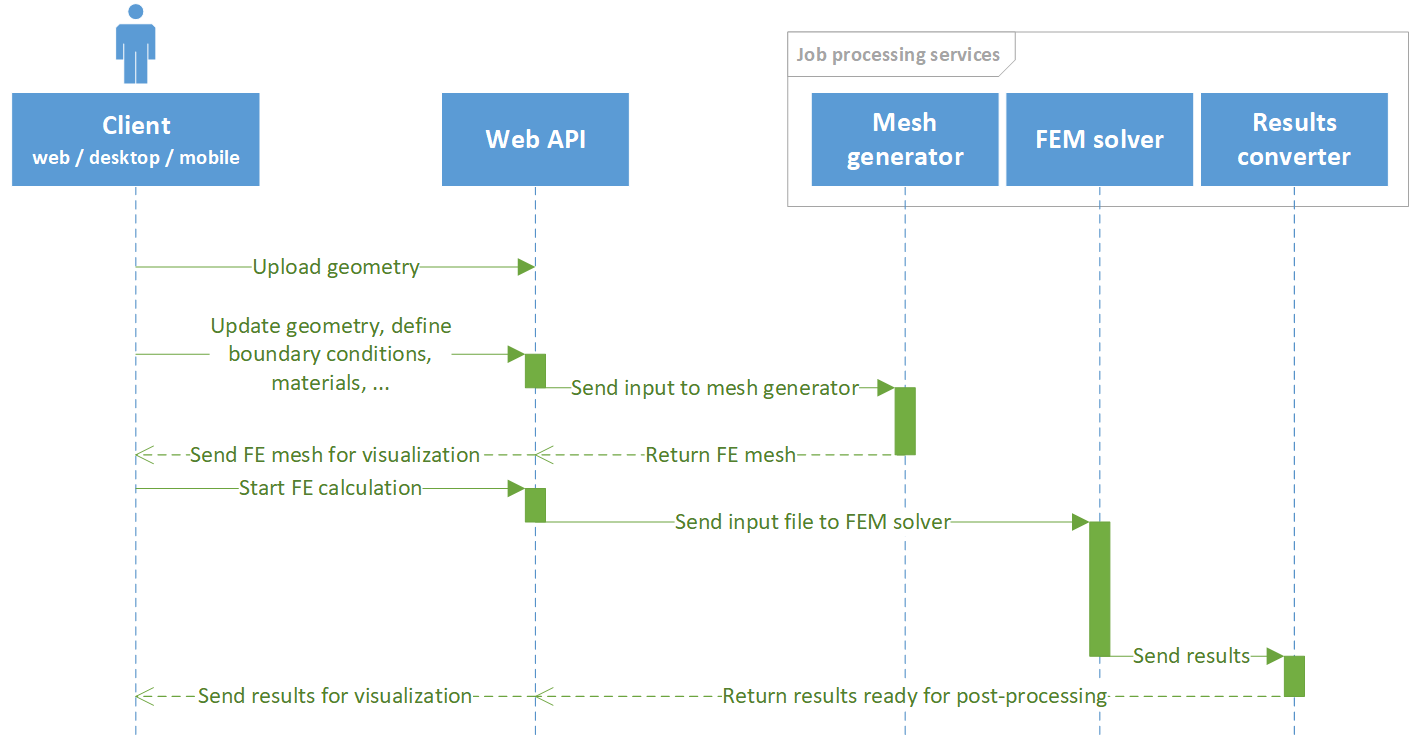
\includegraphics[width=\textwidth]{figures/chapter-data-management/FEA-workflow}
    \decoRule
    \caption{FEA system workflow.}
    \label{fig:FEA-workflow}
\end{figure}

The prototype implementation of the data management system follows the schema and the workflow depicted in Figures \ref{fig:FEA-architecture} and \ref{fig:FEA-workflow}. The difference is that the pre-processing phase is currently excluded. The focus of the work presented in this thesis is primarily on the post-processing features and the representation of results. Therefore, the results from the existing FEM solver are uploaded into the system and the system converts them to the internal representation suitable for post-processing. To test the prototype implementation of the data management system, two client applications are created. The first is the feature-rich desktop post-processor with the support for Microsoft Windows and Linux operating systems. The second is the simple web application that provides basic control over an analysis and basic post-processing capabilities. Its purpose is mainly to demonstrate the benefits of proposed format for storage of results when post-processing complex FEA. Its web-based implementation allows for truly cross-platform experience without the need for installation and it allows to access the analysis data even from low-end mobile devices.

\section{Project-based data representation}
\label{sec:project-db-schema}

Most researchers and engineers typically work independently using their own workstations, while sharing the hardware infrastructure for intensive FEM calculations. The output from the complex analyses are also shared as it would be costly and ineffective if each collaborator had performed her/his own calculations. Since potentially many users can access the server to oversee the analysis and to query the analysis results, a project management scheme is needed. The overall database schema is depicted in Figure \ref{fig:FEA-db-schema}. It is an entity-relationship diagram representing conceptual model that can be mapped on the SQL database model.

\begin{figure}[H]
    \centering
    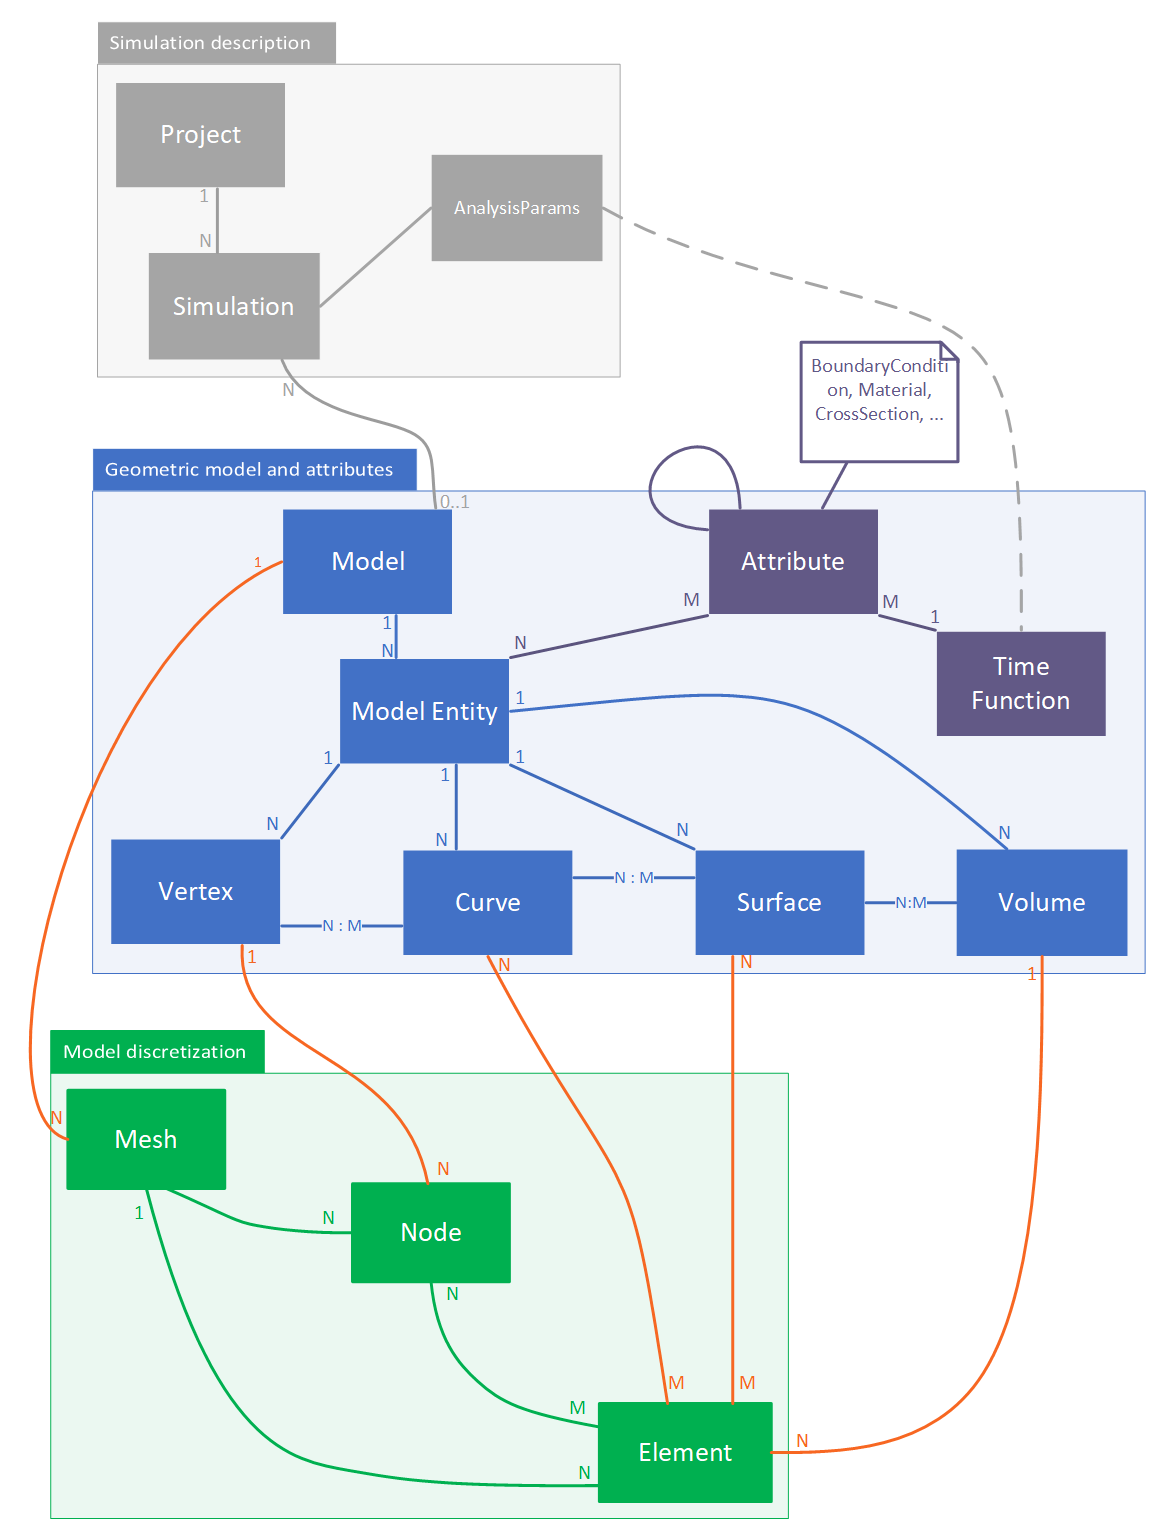
\includegraphics[width=0.8\textwidth]{figures/chapter-data-management/FEA-database-schema}
    \decoRule
    \caption{Database schema for FEA.}
    \label{fig:FEA-db-schema}
\end{figure}

The Project entity holds the basic information about a set of related analyses. It has name, the owner, and the list of other users that have access permissions. The Project has also relations to the list of simulations. The Simulation entity encapsulates the information about a single finite element analysis. Each simulation can have different input -- geometrical model, attributes (properties of model entities, i.e., material properties of volumes, initial and boundary conditions), and/or parameters of analysis (e.g., number of time steps). Geometrical model and its discretizations (finite element meshes) can either be stored directly in a relational database or as a custom file in a blob storage.

% Doplnit tuto kapitolu nejakym textem o projektovych datech / o vstupnim modelu, OOFEM-link, db ...

\section{Storage format for results}
\label{sec:storage-format}

% Pojmout tuto kapitolu jako detailni specifikaci formatu. Inspirovat se dokumentem GiD postprocess format (a take mozna C# proposals na githubu)

The conceptual model presented in Figure \ref{fig:FEA-db-schema} can be naturally extended to contain entities representing the results of the simulations. The project-based data model enhanced with the representation of simulation results is depicted in Figure \ref{fig:FEA-db-schema-results}.

\begin{figure}[H]
    \centering
    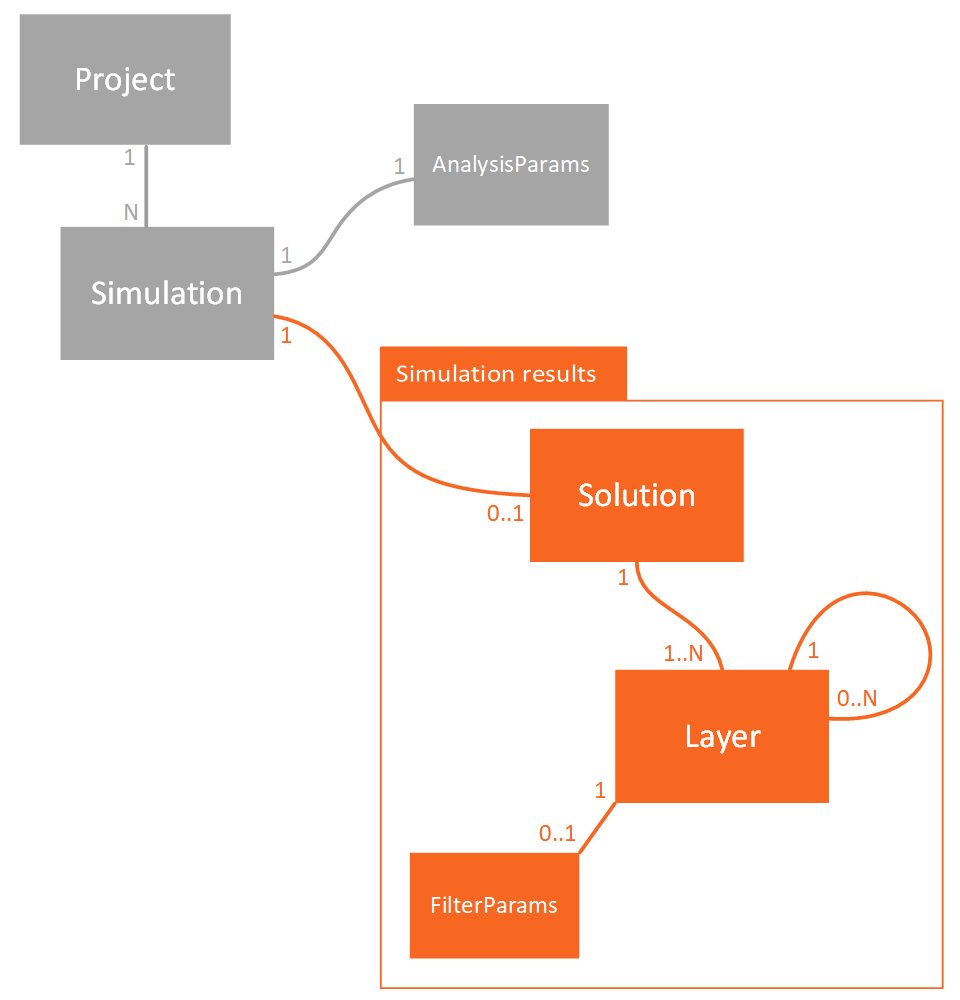
\includegraphics[width=0.6\textwidth]{figures/chapter-data-management/FEA-database-schema-only-results}
    \decoRule
    \caption[Database schema for FEA with results representation only]{Database schema for FEA with results representation only (without the input model).}
    \label{fig:FEA-db-schema-results}
\end{figure}

The simulation results are represented by the Solution entity, which holds a structure representing the results from a FEM solver that are converted to the form suitable for post-processing. The structure has the form of a tree. A node of the tree is represented by the Layer entity. A layer is an association of a mesh and corresponding result fields and other attributes. The use of tree structure allows to preserve the relations between the parent layers and the layers that were derived from them. The mesh that is referenced by a layer need not be the same as the mesh used as the input mesh to the FEM solver. It could be modified by the solver during the calculation, e.g. due to the use of adaptive finite element techniques \footnote{TODO: ... which can automatically refine, coarsen, or relocate a mesh to achieve a solution having a specified accuracy}. Also, the resulting mesh can be further modified to facilitate the post-processor implementation, e.g. the surface representation of a 3D mesh can be generated. Also a number of cross-sections can created at uniform intervals to provide a look inside the mesh. Generally, multiple views on the results can be prepared in advance before the user even starts to investigate the results.

The concept of a layer is not new. It is used in existing implementations of the post-processors in FEA software packages (often named \textit{filter} instead of layer), to represent a view on the results. However, the layers (visual filters) are usually generated on demand by specific user request and they are not kept in a persistent storage. The proposed storage format for results is built on top of layer tree structure directly, which allows layers to be accessed later on, even on a different device, or shared by multiple users working on the same project.

In the prototype implementation of the FEA data management system, it is supposed that the FEM solver uses its own proprietary format to represent the result from the simulation. As the system is designed to be independent of individual components, the Results converter component converts the results from the FEA solver into the standardized layer-based format suitable for post-processing. The specification of the format follows.

\subsection{Format specification}

All documents that participate in the storage format are presented in JSON format. JSON is the today's standard for data transport in web technologies and also as a storage format in currently popular NoSQL\footnote{TODO: NoSQL ... Stands for Not-only SQL ...} databases. It is a consise textual format easily readable both for a human and for a computer. However, the storage format is not tightly coupled with JSON, data can be encoded in another structured format, such as XML. Also, as mentioned above in the text, there are two types of locations the data can be stored in -- \textbf{remote} and \textbf{local}. Both locations are supported in the prototype implementation. In either case the key part of the format is a solution document. An example of the solution document is given in Listing \ref{lst:solution.json}. In case of the remote storage, the solution document is stored in a relational database as part of the project-based data representation shown in Figure \ref{fig:FEA-db-schema-results}, while the rest of documents are stored in a blob storage as group of JSON documents. In case of the local storage, all documents, including the solution, are stored in a folder as JSON files in local file system on a personal computer on which the results are post-processed.

As can be seen in the example of the solution document in Listing \ref{lst:solution.json}, each layer is assigned a unique identifier, specifically a GUID\footnote{TODO: GUID... Globally unique identifier, sometimes the term UUID is used ... 128bit, 4bits reserved for version ...} number. A GUID in its textual representation is also used to unambigously determine the location of the layer documents. In case of a solution stored locally, a GUID is used as a name of the folder the related layer documents are stored in. For remote solutions, a GUID is used as a part of a URL when requesting resources from a database or a blob storage.

% TODO: describe properties in solution document? Id, ProjectName, Location, Results, Layers, Layers.Id, Layers.Name, Layers.FilterType, Layers.Children

Data in each layer are stored in four types of documents.
\begin{itemize}
    \item \textbf{Summary document} contains all the descriptive information about the layer. An example of a summary document in JSON format is presented in Listing \ref{lst:summary.json}. Besides a unique id, a layer has its name, which the user can choose arbitrarily, otherwise it is automatically derived from the \code{Filter} property. \code{Filter} property describes the parameters of the transformation applied to the parent layer to obtain the current layer. \code{ParentId} property contains the GUID assigned to the parent layer. The topmost root of the layer tree has no parent. Therefore, its \code{ParentId} property is null as well as \code{Filter} property. Default name for the root layer is ``master''\footnote{The format allows the existence of multiple \textit{master} layers, but it turns out that it is not necessary in practice. In the vast majority of cases, there is a single root layer and it is called ``master''.}.

    \code{Meshes} property holds a collection of mesh descriptors. A mesh descriptor serves as an reference to an actual mesh document related to a layer. Each mesh in a layer is assigned an index. It is a number that uniquely identifies the mesh within the layer. \code{TimeSteps} property of each mesh contains the list of time steps for which the mesh is defined. In usual case there is only one mesh for all time steps. In some cases, however, there can be different mesh for each time step. Application of deformation filter on a layer yields a derived layer that contains the same number of meshes as is the number of time steps, because the deformed meshes are generated by translating the nodes of the parent mesh by displacements calculated for each time step. Even the master layer can be composed of multiple meshes, e.g. when representing the results from a simulation of construction stages. The time step number must be a unique floating-point number as it serve as an identifier.
    
    Each mesh has optional set of attributes. An attribute is an umbrella term for additional information assigned to mesh entities. It is usually a property of the input model that is propagated to the results as it can be interesting during post-processing. The most common attribute is the material number that is assigned to each element of the mesh.

    \code{Fields} property contains a dictionary of result descriptors. Each field descriptor is introduced by the name of the field imported from the FEM results. Field can be composed of one or more components. Similarly, each component descriptor is identified by its name and enumerates the time steps in which the component is defined. Each time step descriptor contains the index of the corresponding result document as well as the index of the mesh document. Each result document always contains data for only one data component. However, the format allows that the data from multiple time steps can be gathered and stored in a single result document. The compression can be then applied on the range of time steps as a whole to achive better compression ratio. Therefore, to recover an arbitrary data component located either in a local or in a remote storage, the post-processor needs just a triplet of identifiers -- the layer id, the index of result document, and the time step.

% TODO: summary document muze take volitelne obsahovat property MeshFallbackLayerId, AttributeFallbackLayerId, a DataFallbackLayerId - vyuzito napr pro deformacni vrstvu - nemusi se kopirovat data

    \item \textbf{Mesh document} contains the geometric representation of a finite element mesh. An example of a mesh document in JSON format is presented in Listing \ref{lst:mesh.json}. Positions of the nodes are encoded in \code{PointCoordinates} property\footnote{Note that the terms \textit{node} and \textit{element} are internally referred to by more general terms \textit{point} and \textit{cell}.\label{foot:points-cells}}. Position of each node is a vector, whose components are floating-point numbers. Number of vector components is equal to the number of dimensions of the mesh. Vector components are flattened into a one dimensional array and converted to text using binary-to-text encoding (more about encoding in Section \ref{subsec:encoding}). \code{CellConnectivity} property\footnotemark[\getrefnumber{foot:points-cells}] contains encoded list of indices of element nodes that point to the coordinate array. The number of nodes per element can be retrieved by decoding \code{CellTypes} property, in which the types of all elements are stored. The supported element types along with their identifiers are depicted in Figure \ref{fig:supported-cell-types}. The identifiers are 8-bit unsigned integers (bytes) and the values match the definition of cell types in VTK file format \cite{XXX-vtk-file-format-pdf} to provide basic compatibility and to ease the conversion from the VTK format.
    
    \begin{figure}[H]
        \centering
        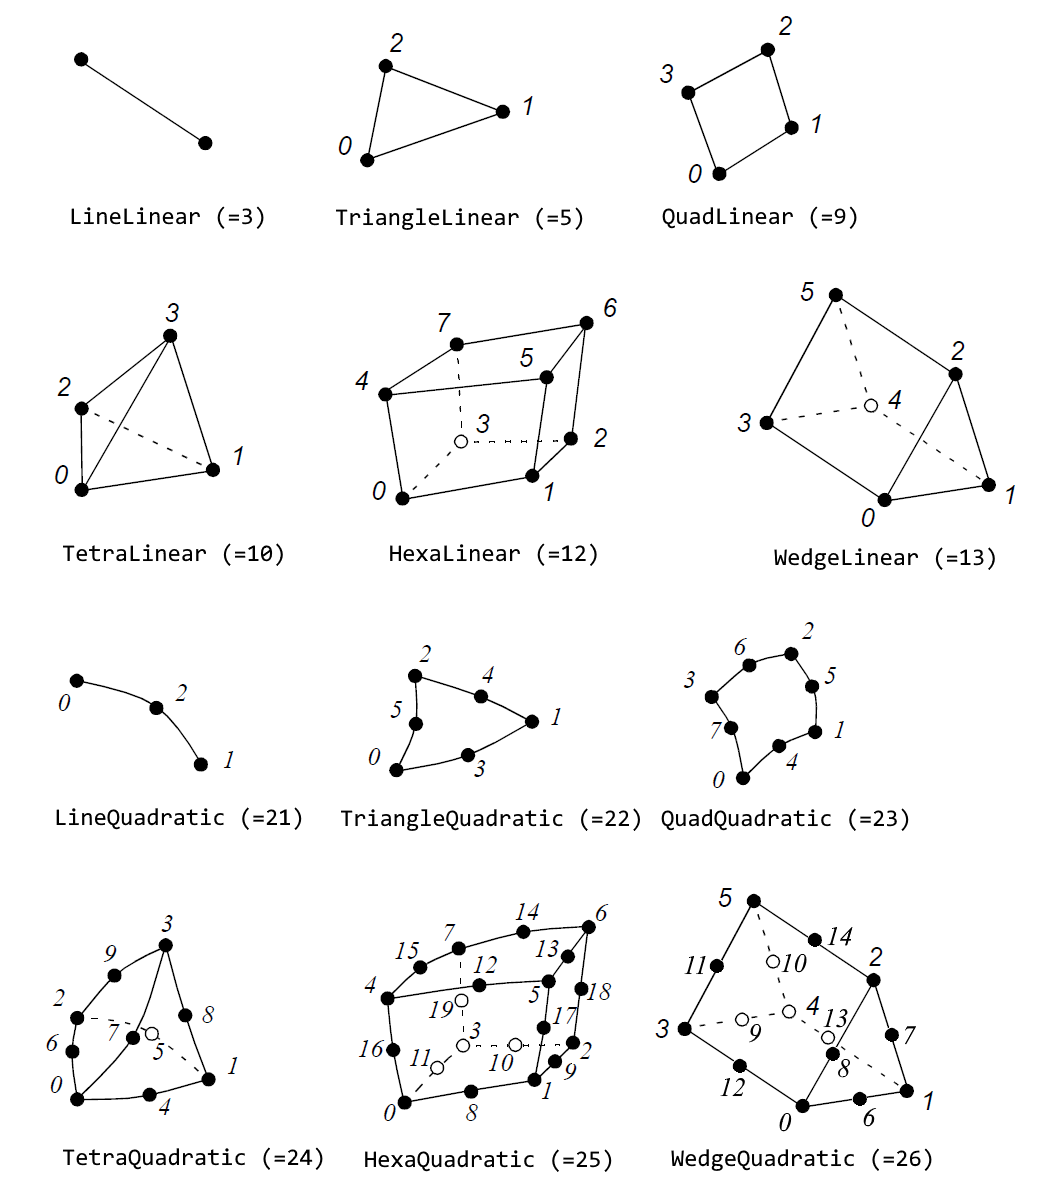
\includegraphics[width=0.9\textwidth]{figures/chapter-data-management/supported-cell-types}
        \decoRule
        \caption[Element types supported in storage format]{Element types supported in storage format. The values used for encoding element types in CellTypes array are shown in parentheses. The illustrations of elements are taken from \cite{XXX-vtk-file-format-pdf}.}
        \label{fig:supported-cell-types}
    \end{figure}
    
    Properties \code{Center} and \code{Radius}, eventhough their values can be calculated from the coordinate array, were added as an performance optimization for a post-processor since it is usually needed to normalize the mesh dimensions before the first rendering.

    \item \textbf{Attribute document} --- ... An example of a attribute document in JSON format is presented in Listing \ref{lst:attribute.json}.

    \item \textbf{Result document} --- ... An example of a result document in JSON format is presented in Listing \ref{lst:result.json}.

    % result.json, attribute.json - popsat data location: Points/CellPoints/Cells (jak je to z extrapolaci z gaussovych bodu?)
    % je nutne zachovat 1:1 mapovani vysledku na sit, kvuli efektivni implementaci postprocessoru
\end{itemize}

% shrnout proc je to vyhodne mit to takto rozdelene do jednotlivych souboru. vypada to divoce a slozite, nektere info je zduplikovane, proc je to lepsi nez mit to v jednom souboru? Vyssi efektivita, jednodussi implementace postprocessoru, data jsou predpripravena, rovnou se pouziji jako buffery v opengl

% popsat, jak jsou soubory/bloby pojmenovane - index je soucasti souboru. Cesta k danemu souboru je tedy .../{Guid}/{index}.{file-type}.json. Nebo dat az do kapitoly Implementation details?

\subsection {Compression}
% Compression methods: SVD, Wavelet, polynomial functions, ... Kazdou rozepsat, u Wavelet zminit Hilbert curve?
% main features for optimization: key time steps (time step span compression), Randomized SVD, Parallelization, Sparse matrix of details, prenasobeni U matice singularnimi cisly, trochu usetrim pamet, mohu pouzit vzorkovani...
% format is designed to be open for other compression methods in the future...

% See chapter \ref{chapter:SVD}

\subsection {Encoding}
\label{subsec:encoding}
% base64, JSON, XML, zkracovani datovych poli u meshe a u dat. u meshe se to zkracuje jinak.

\section{Post-processing}
\label{sec:postprocessing}

Typical layer tree consist of the master layer and zero or more derived layers. The layer tree corresponding to the example of the solution document in Listing \ref{lst:solution.json} is also shown in Figure \ref{fig:layers-tree}. The master layer is ... Children represent the visual filters applied on the master layer

\begin{figure}[H]
    \centering
    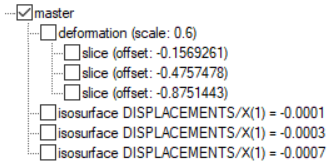
\includegraphics[width=0.5\textwidth]{figures/chapter-data-management/layers-tree-diagram}
    \decoRule
    \caption{Diagram of layer tree.}
    \label{fig:layers-tree}
\end{figure}


% V teto kapitole popsat navrh post-processoru, ktery je postaven na popsanem datovem formatu
% layers, filters, vytvoreni Surface vrstvy pro webovy postprocessor, barevna skala, prepinani skalarnich velicin, vektorove veliciny - je treba nacist vice komponent najednou. Dekomprese: prenasobeni matic - staci jeden radek. ...

% ke kazdemu typu filtru pridat obrazek z postprocessoru at je to zajimavy

Displacement in Z axis: Figure \ref{fig:beam-master-layer} and Figure \ref{fig:beam-deformation-layer}.

Displacement in X axis: Figure \ref{fig:beam-slice-layers} and Figure \ref{fig:beam-isosurface-layers}.

\begin{figure}[H]
    \centering
    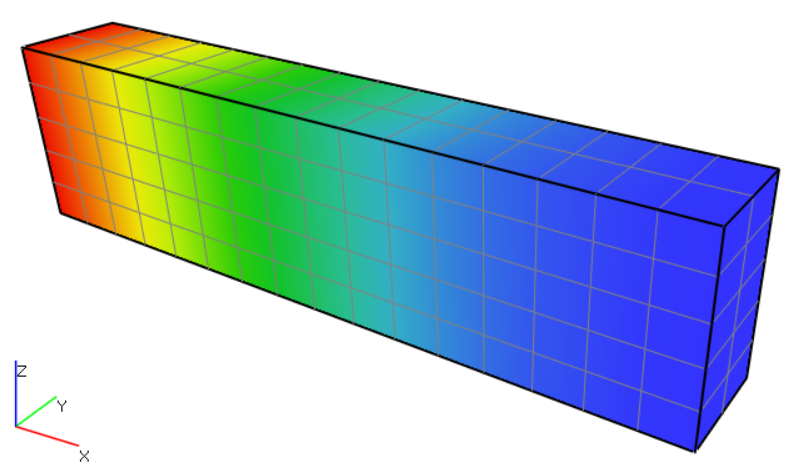
\includegraphics[width=0.7\textwidth]{figures/chapter-data-management/beam-master-layer}
    \decoRule
    \caption{Example of the master layer visualization.}
    \label{fig:beam-master-layer}
\end{figure}

\begin{figure}[H]
    \centering
    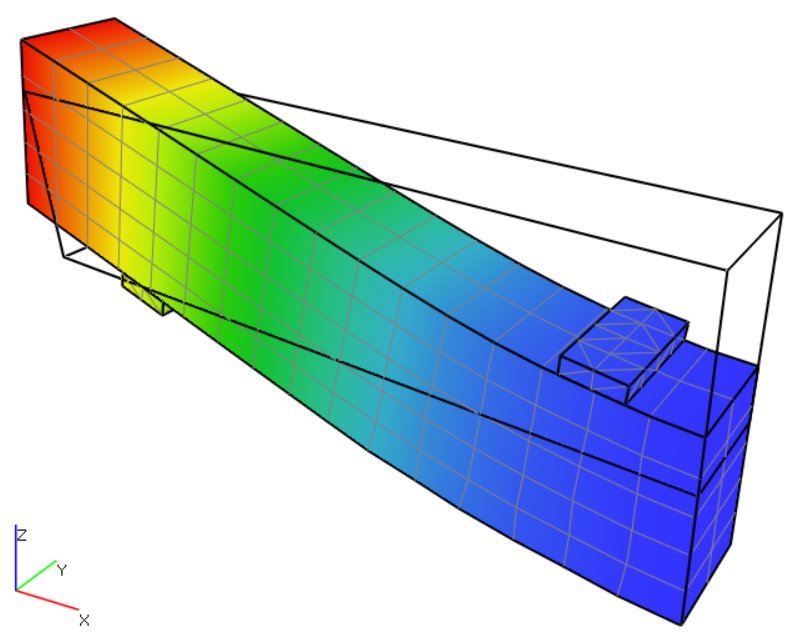
\includegraphics[width=0.7\textwidth]{figures/chapter-data-management/beam-deformation-layer}
    \decoRule
    \caption{Example of the deformation layer visualization.}
    \label{fig:beam-deformation-layer}
\end{figure}

\begin{figure}[H]
    \centering
    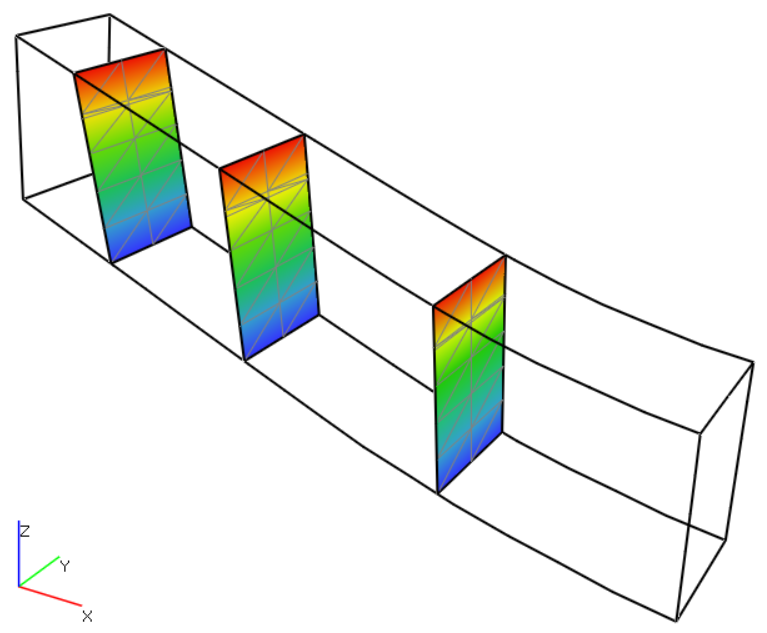
\includegraphics[width=0.7\textwidth]{figures/chapter-data-management/beam-slice-layers}
    \decoRule
    \caption{Example of multiple slice layers.}
    \label{fig:beam-slice-layers}
\end{figure}

\begin{figure}[H]
    \centering
    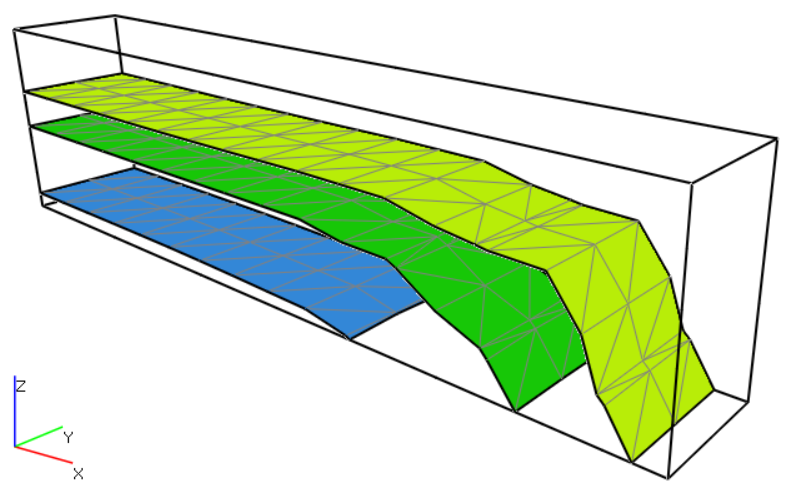
\includegraphics[width=0.7\textwidth]{figures/chapter-data-management/beam-isosurface-layers}
    \decoRule
    \caption{Example of multiple iso-surface layers.}
    \label{fig:beam-isosurface-layers}
\end{figure}


\section{Implementation details}
\label{sec:implementation-details}

% implementation details; cloud-infrastructure, Azure functions, web frontend, backend providing project info, blob-storage with layer format; command-based console management - popsat prikazy; reference to appendix with storage format examples
% Jak probiha komunikace s API a dotaz na vrstvy. Jak funguje RemoteSolutionController. Remote/Local solutions - neni rozdil, postprocessor je tenky klient
% SVD compression using redsvd; How is realized postprocessing of compressed data
% Encoding: converting to text representation, base64, NaN values, ... UTF8
% Calculating CellOffsets from CellConnectivity and CellTypes

% Webový browser, WebGL, textové pole se zadáváním příkazů, veškeré zpracování příkazů na serveru, na klient se budou posílat jen grafické buffery

% Přidat podkapitolku o implementaci barevné škály (diskrétní, spojitá, isoareas shader)

Figure \ref{fig:results-class-diagram} ...

% TODO: do results class diagramu pridat pole FallBackLayerId a pak ho v textu popsat
% TODO: zminit optimalizaci v layer tree structure - sdileni dat u vrstev, ktere maji kompatibilni sit - napriklad Deformation filter - je tam odkaz na 

\begin{figure}[H]
    \centering
    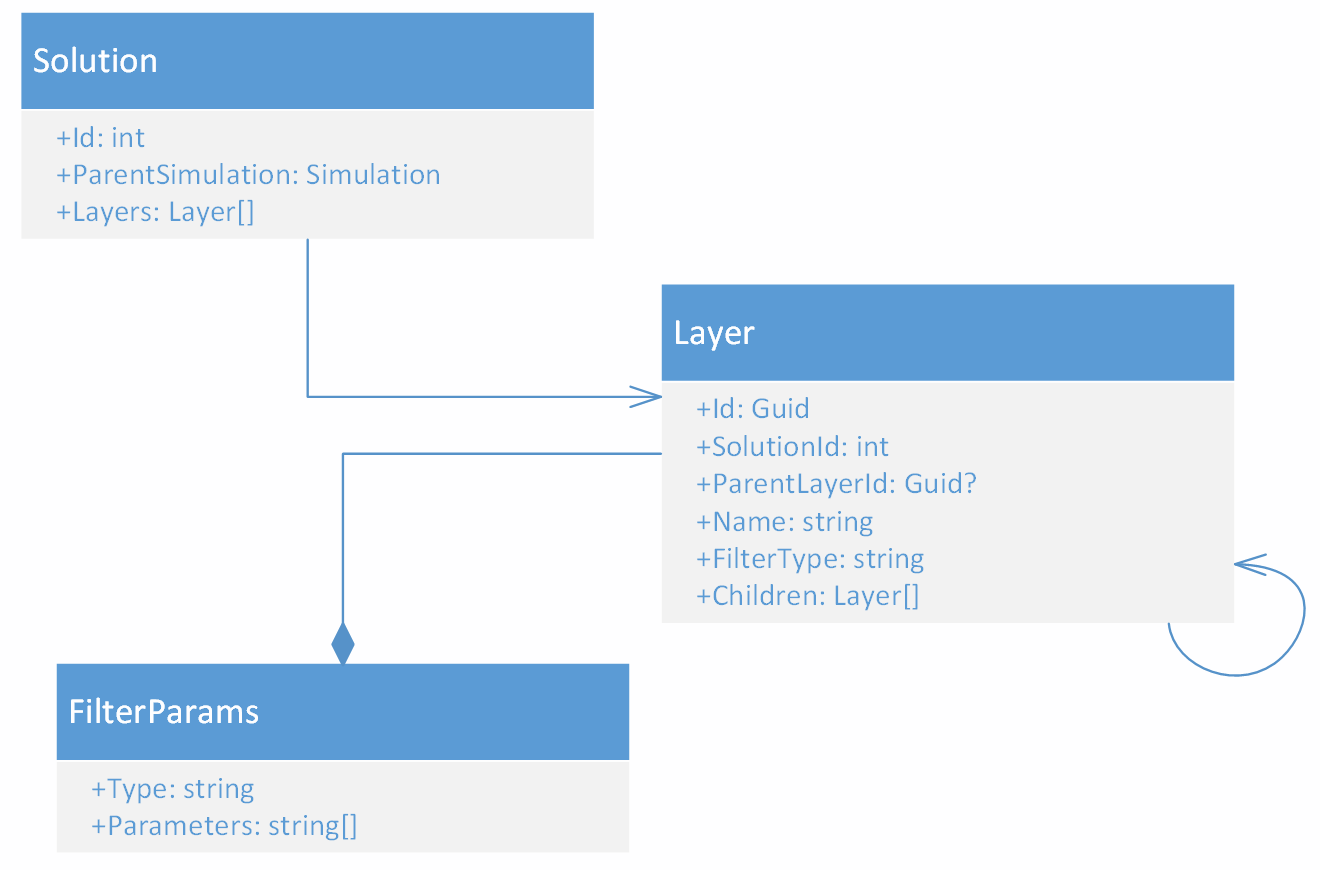
\includegraphics[width=0.7\textwidth]{figures/chapter-data-management/results-class-diagram}
    \decoRule
    \caption{Class diagram of results representation}
    \label{fig:results-class-diagram}
\end{figure}